\section*{Комментарии и ссылки}

\subsubsection*{Ангел и Дьявол Конвея}

Недавний доклад об этой увлекательной головоломке содержится в очень симпатичной коллекции под редакцией Ричарда Новаковского.\footnote{\emph{Games of No Chance.} Edited by Richard Nowakowski, Cambridge University Press, Cambridge, 1996. \href{http://library.msri.org/books/Book29/}.} 

Элвин Берлекэмп,  показал, что если Ангел обладает «силой 1», то есть может делать только одиночные ходы короля, то Дьявол побеждает.
Может оказаться, что Дьявол побеждает независимо от силы Ангела; 
однако, похоже на то, что силы 2 достаточно для того, чтобы Ангел выжил.

Ангел силы 1000 должен быть в состоянии выжить, но, как отмечает сам изобретатель головоломки Джон Конвей в своей статье, есть несколько раздражающих нюансов, которые, возникают на пути к решению.
Один нюанс заключается в том, что Дьявол не может ошибиться;
то есть независимо от того, какую клетку он уничтожит, полученная конфигурация будет для него лучше чем начальная.
Другой нюанс заключается в том, что Дьявол, кажется, имеет ответ на любую разумную стратегию «потенциальной функции», которую может использовать Ангел, которая говорит ему, куда ходить в зависимости от того, какие клетки уничтожены. %???

Кроме того, если Ангел имеет какие-то, казалось бы, легкие недостатки вроде того, что ему запрещено ступать на клетку в далее чем $10^{99}$ клеток к югу от клетки на, которой он побывал, то Дьявол побеждает.

Сам Конвей до сих пор верит в Ангела, о чём свидетельствует тот факт, что он предлагает приз в 1000 долларов за доказательство того, что Дьявол побеждает, но только 100 за стратегию для достаточно сильного Ангела.

??? Задача решена ???

\subsubsection*{$\bm{3x+1}$ дилемма}

Мало что известно об источнике этой знаменитой головоломки, также известной как гипотеза Коллатца, сиракузская задача, задача Какутани, алгоритм Хасса и гипотеза Улама.
1 июля 1932 года, студент Гамбургского университета по имени Лотар Коллатц записал похожую задачу в свою тетрадь, но задача известная теперь, кажется, стала популярна только в 1950-е годы.

Джефф Лагариас из лабораторий AT\&T написал очень хороший обзор на эту тему.\footnote{Jeff Lagarias, ``The 3x + 1 Problem and its Generalizations'', Amer. Math Monthly, Vol. 92 (1985), pp. 3--23, \href{http://www.cecm.sfu.ca/organics/papers/lagarias/}{www.cecm.sfu.ca/organics/papers/lagarias/}.}

Лагариас указывает на то, что эта головоломка, упоминалась как часть заговора с целью замедлить математические исследования в США.
Пусть это будет предупреждение!

\subsubsection*{Самая длинная общая подпоследовательность}

Эта задача известна как минимум с 30-ых годов; она упоминается в диссертации В. Данчика 1974 года защищённой в Уорикском университете.
Майкл Стил (Пенсильванский университет) сформулировал гипотезу, что $C_{1/2} = 2/(1+\sqrt{2})\approx 0{,}828427$.
Вацлав Хватал и Давид Санкофф показали, что $0{,}773911 < C_{1/2} < 0{,}837623$, и это дало основание предполагать что число Стила слишком велико;
в конце концов Джордж Люкер (Калифорнийский университет в Ирвайне) убил гипотезу в 2003 году, доказав, что $0{,}7880 < C_{1/2} < 0{,}8263$.\footnote{\textit{Proc. 14th ACM-SIAM Symp. on Discrete Algorithms,} Baltimore, Maryland, 2003, pp. 130--131.}

Существование $C_p$ легко следует из субаддитивности,\footnote{см., например, Rick Durrett, \textit{Probability: Theory and Examples,} Wadsworth, 1991, Section 6.6.} но это не позволяет вычислить саму константу.
Другой такой пример: Бела Боллобаш и я доказали существование числа $K_d$ такого, что самая длинная координатно-возрастающая цепь среди $n$ случайных точек в $d$-пространстве имеет размер около $K_d\cdot n^{1/d}$.
Мы знаем, что $K_1=1$, $K_2=2$ и $\lim_{d\to\infty} K_d=e$, но не знаем чему равно $K_3$.

Если мы варьируем вероятность $p$ единиц при $p > 1/2$, мы, конечно, получаем, что $C_p>p$, так как мы можем смотреть на подпоследовательности, состоящие только из единиц.
Таким образом, $C_p\to 1$ при $p\to 1$, и это даёт основание предполагать, что $C_p$ минимально при $p=1/2$.
Чтобы это доказать, нам не обязательно знать точные значения $C_p$,
но, на данный момент, никто не знает, как это сделать. %???коряво

\subsubsection*{Квадратура озера}

Хорошее обсуждение этой головоломки дано на «Геометрической свалке» Давида Эпштейна.%
\footnote{\href{http://www.ics.uci.edu/~eppstein/junkyard/jordan-square.html}{www.ics.uci.edu/~eppstein/junkyard/jordan-square.html}}
Похоже, что есть доказательства того, что квадрат можно вписать во все достаточно гладкие замкнутые плоские кривые.%
\footnote{Например Walter Stromquist, ``Inscribed Squares and Square-Like Quadrilaterals in Closed Curves,'' Mathematika, Vol. 36 (1989), No. 2, pp. 187--197}
Тем не менее в общем случае гипотеза остается открытой уже более 90 лет.
\footnote{Victor Klee and Stan Wagon, ``Old and New Unsolved Problems in Plane Geometry and Number Theory,'' Mathematical Association of America, 1991.}

\medskip

Немного неловко, что математики не могут понять, можно ли вписать квадрат в любую замкнутую плоскую кривую, не так ли?

\subsection*{Одинокий бегун}

Эта замечательная гипотеза, по-видимому, поставлена Дж. М. Уиллсом.%
\footnote{J. M. Wills, ``Zwei Satze uber Inhornogene Diophantische Approximation von Irrationalzahlen,'' Monatsch. Math., Vol. 71 (1967), pp. 263-269.}
В 1973 году, независимо её сформулировал Т. В. Кусик.
В 1984 году, вместе с Карлом Померанием они доказали гипотезу для не более чем пяти бегунов.
Том Бохман, Рон Хольцман и Дэн Клейтман (те самые, что из ящиков и подъящиков) доказали её для шести,
\footnote{Bohman, Tom; Holzman, Ron; Kleitman, Dan
``Six lonely runners.''
Electron. J. Combin. 8 (2001), no. 2.\\
\href{https://www.combinatorics.org/ojs/index.php/eljc/article/view/v8i2r3/pdf}{www.combinatorics.org/ojs/index.php/eljc/article/view/v8i2r3/pdf}}
есть также более короткое доказательство Джерома Рено.\footnote{Renault, J\'{e}r\^{o}me ``View-obstruction: a shorter proof for 6 lonely runners.'' Discrete Math. 287 (2004), no. 1-3, 93--101.}

\medskip

Название головоломке дано Луисом Годином из Университета Саймона Фрейзера, который также внёс вклад. %???коряво

Головоломка носит численно-теоретический характер; можно доказать, что достаточно рассмотреть случай когда все скорости являются целыми.

\subsubsection*{Разбор пар в корзинках}

Эта любопытная задачка возникла в Bellcore (ныне iconectiv) в связи со статистическими исследованиями, предполагающими предпочтения заказов с связями.
Я работал над ней с коллегами Майклом Литтманом (ныне в Рутгерсе) и Грэмом Бригиттом (Лондонская школа экономики).
Задача обобщается не только на $k$ шаров в каждой корзинке, но и на корзинки с разным числом шаров.
Мы сосредоточимся только на корзинках с двумя шарами в каждой.

Если бы у нас было $n$ корзинок с $n$ шарами, по одному в каждой и пронумерованных в обратном порядке, то это стандартное и простое упражнение, чтобы понять, что $\binom{n}{2}$ перекладываний необходимы для того, чтобы каждый шарик попал в свою корзинку.
Один из способов это увидеть --- смотреть за числом пар находящихся в обратном порядке, заметив, что одно перекладывание исправляет только одну пару.
Это также говорит о том, что если мы не делаем глупостей (а именно, не меняем два шара, которые уже находятся в правильном порядке), то нам потребуется ровно $\binom{n}{2}$ перекладываний.
Более того, независимо от начальной конфигурации, $\binom{n}{2}$ перекладываний достаточно --- обратный порядок, с которого мы начали, это, как и следовало ожидать, худший случай.

Похоже, те же рассуждения работают и с двумя шарами в каждой корзинке.
Можно представить, что у нас шары двух цветов, красные и зелёные, и шары одного цвета пронумерованы от $1$ до $n$; 
если отдельно сортировать каждый набор, то мы закончим за $2\binom{n}{2}$ шага.
Наверняка $2\binom{n}{2}$ шагов необходимо, верно?

А вот и нет!
Рассмотрим случай $n = 5$ и посмотрим на приведенную ниже диаграмму --- волшебным образом мы отсортировали шары только за 15 переклдываний, вместо 20, которые казались нам необходимыми.

\begin{figure}[h!]
\centering
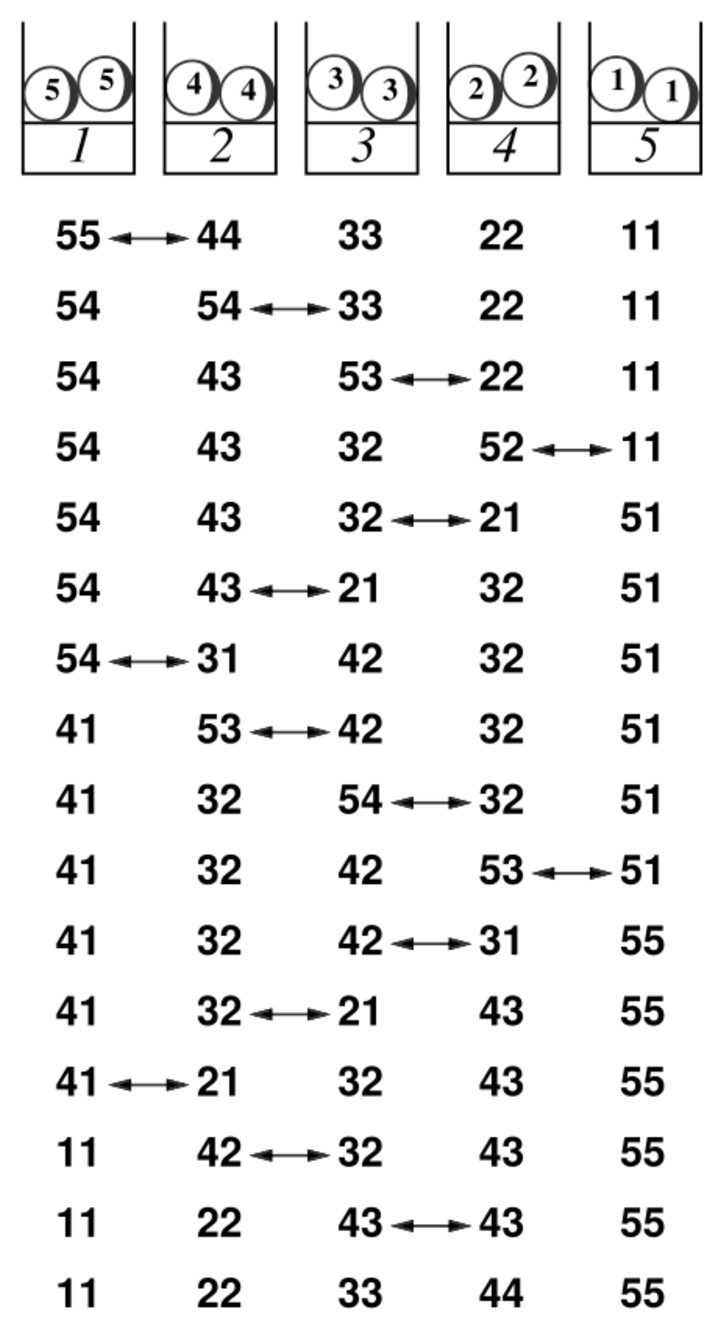
\includegraphics[scale=0.5]{Figs/UnsolvedPuzzles/5bin}
\end{figure}

Нельзя сделать лучше, чем 15 перекладываний; более того необходимо $\lceil\binom{2n}{2}/3\rceilr$ перекладываний для упорядочивания n двухшаровых корзинок.
Чтобы увидеть это, присудите 1 балл за пас, то есть шар с высоким номером, проходящий слева от шара с низким номером вправо.
Мы назначаем по 1/2 балла за догон и движение дальше, если прохождение делается в два этапа.
Кроме того, два счетчика с одинаковым числом должны нести 1-точечный заряд, поскольку они должны отделяться (1/2 точку) в какой-то точке, а затем рекомбинироваться.
Поэтому есть (22 ") точки, которые надо собирать в процессе сортировки всех шариков.

За один шаг, о каком количестве моментов можно позаботиться?
Предположим, что шарики с номерами u и y обмениваются между бункером, содержащим u и v, и смежным бункером, содержащим x и y.
Мы можем получить 1 балл за u против y, 1/2 каждый за u против v (за "движение дальше") и y против x, и 1/2 каждый за него против x (за "догоняющий") и y против vt в общей сложности за 3 очка.
Далее следует привязка.

Есть еще хорошие новости. Как и в случае с ячейками размера 1, нетрудно показать, что изменение порядка снова является самым сложным случаем; Таким образом, если/2 (") является минимальным количеством свопов, необходимых для сортировки n ячеек и двух шариков в ячейку, из любой начальной конфигурации, то для этой головоломки необходимо J2 (^).
Также легко доказать, что если обмен должен быть сделан между ячейками i и i 1, то не может быть неправильным заменять самый высокий пронумерованный шар в ячейке i с самым низким пронумерованным шаром в ячейке t 1.

Но есть плохие новости, или загадки не было бы в этой главе. Ограничение | "(^)/3l не всегда достижимо; Например, это показывает, что/2 (G) > 21, но на самом деле компьютерный поиск не нашел способа сделать корпус из шести бункеров менее чем за 22 свопов. Хуже того, хорошо выглядящий своп, показанный на диаграмме для пяти бункеров, обычно не является оптимальным.

Но вполне возможно, что какая-то другая схема оптимальна, и, возможно, даже обеспечивает хорошую формулу для f2 (p) *
